\documentclass[a4paper, 11pt]{article}
\usepackage{lipsum} %This package just generates Lorem Ipsum filler text. 
\usepackage{fullpage} % changes the margin
\usepackage{mathpazo}
\usepackage{multicol}
\usepackage{graphicx}
\usepackage{enumerate}
\usepackage{amsmath,amsfonts,amsthm} % Math packages
\usepackage{listings}
\usepackage{matlab-prettifier}

\begin{document}
%Header-Make sure you update this information!!!!
\noindent
\large\textbf{Homework 8} \hfill \textbf{Hongyu Yan (516030910595)} \\
\normalsize {\bf CS 259 Numerical Methods for Data Science} \hfill ACM Class, Zhiyuan College, SJTU\\
Prof.~{\bf David Bindel} \hfill Due Date: July 7, 2018\\
TA.~{\bf Yurong You, Xinran Zhu} \hfill Submit Date: \today

\section*{Problem 1}

\subsection*{1.1}
First, we can prove that 0 is an eigenvalue of $L$, with an associated eigenvector of all ones:
$$
L\begin{bmatrix}
1 \\ 1 \\ \vdots \\ 1
\end{bmatrix}
=
\begin{bmatrix}
-\sum_{j!=1}w_{1j} & w_{12} & \cdots & w_{1m} \\
w_{21} & -\sum_{j!=2}w_{2j} & \cdots & w_{2m} \\
\vdots & \vdots    &          \ddots & \vdots \\
w_{m1} & w_{m2} & \cdots & -\sum_{j!=m}w_{mj} \\
\end{bmatrix}
\begin{bmatrix}
1 \\ 1 \\ \vdots \\ 1
\end{bmatrix}
=
\begin{bmatrix}
0 \\ 0 \\ \vdots \\ 0
\end{bmatrix}
$$
So 0 is an eigenvalue of $L$, with an associated eigenvector of all ones.

Second, we need to prove all eigenvalues of $L$ are non-negative. In other words,
we need to prove $L$ is positive semi-definite.

We can define M as 
$$
M_{ke} = \left\{
\begin{aligned} 
\sqrt{w_{ij}}, &  & e = i \\
-\sqrt{w_{ij}}, &  & e = j \\
0, &  & otherwise
\end{aligned}
\right.
$$
where k means the k-th edge in the graph connecting vertex i and j.

So we have $L = M^TM$, which means L is positive semi-definite.

\subsection*{1.2}
The MATLAB code is as below:
\begin{lstlisting}[language = Matlab, numbers=left,   
  numberstyle=\tiny,keywordstyle=\color{blue!70},  
  commentstyle=\color{red!50!green!50!blue!50},frame=shadowbox,  
  rulesepcolor=\color{red!20!green!20!blue!20},basicstyle=\ttfamily,
  tabsize=2]
% routine to construct W
% y is a m*3 matrix, eps is the threshold
m = 5;
eps = 0.8;

x = rand(m, 2);
y = f(x);
W = zeros(m, m);
for i = 1:m
	for j = 1:m
		W(i,j) = norm(y(i,:) - y(j,:), 2);
		if (W(i,j) > eps)
			W(i,j) = 0;
		end
	end
end

D = diag(sum(W,2));
L = D - W;
[V, U] = eig(L);
u2 = U(2, 2);
u3 = U(3, 3);
v2 = V(:, 2);
v3 = V(:, 3);
B = [v2 / sqrt(u2) v3 / sqrt(u3)]
\end{lstlisting}
$$
W =
\begin{bmatrix}
         0 &       0 &  0.7269 &  0.2319 &  0.3749 \\
         0 &       0 &  0.4990 &       0 &       0 \\
    0.7269 &  0.4990 &       0 &       0 &       0 \\
    0.2319 &       0 &       0 &       0 &  0.2462 \\
    0.3749 &       0 &       0 &  0.2462 &       0
\end{bmatrix}
$$
$$
\hat{X} =
\begin{bmatrix}
    0.0882 &   0.2937 \\
   -1.3032 &  -0.2874 \\
   -0.6102 &   0.1504 \\
    1.0237 &  -0.8239 \\
    0.8014 &   0.6673
\end{bmatrix}
$$
\section*{Problem 2}
The MATLAB code is as below:
The MATLAB code is as below:
\begin{lstlisting}[language = Matlab, numbers=left,   
  numberstyle=\tiny,keywordstyle=\color{blue!70},  
  commentstyle=\color{red!50!green!50!blue!50},frame=shadowbox,  
  rulesepcolor=\color{red!20!green!20!blue!20},basicstyle=\ttfamily,
  tabsize=2]
m = 5;
eps = 0.8;
X = rand(m, 2);
Y = f(X);

W = zeros(m, m);
for i = 1:m
	for j = 1:m
		W(i,j) = norm(Y(i,:) - Y(j,:), 2);
		if (W(i,j) > eps)
			W(i,j) = 0;
		end
	end
end

N = floyd_warshall(W);
J = eye(m, m) - ones(m, m) / m;
B = -0.5 * J * (N .* N) * J';
[V, U] = eig(B);
v1 = V(:,1);
v2 = V(:,2);
u1 = U(1, 1);
u2 = U(2, 2);
Iso = [v1*sqrt(u1) v2*sqrt(u2)]  
\end{lstlisting}
$$
W =
\begin{bmatrix}
         0 &       0 &       0 &  0.7570 &       0 \\
         0 &       0 &  0.3191 &  0.1799 &       0 \\
         0 &  0.3191 &       0 &  0.3374 &  0.5994 \\
    0.7570 &  0.1799 &  0.3374 &       0 &  0.7371 \\
         0 &       0 &  0.5994 &  0.7371 &       0
\end{bmatrix}
$$
$$
\hat{X} =
\begin{bmatrix}
   -0.8167 &   0.1905 \\
   -0.0329 &  -0.3209 \\
    0.2289 &  -0.1372 \\
   -0.0547 &   0.0058 \\
    0.6753 &   0.2618
\end{bmatrix}
$$

\section*{Problem 3}
\subsection*{3.1}
Thin plate spline from $\mathbb{R}^2$ to $\mathbb{R}$ is:
$$
\hat{f}(x)=\sum_{j=1}^mc_j\|x-x_j\|log\|x-x_j\|+d_1+d_2x(1)+d_3x(2)
$$
$x(1)$ means its first dimension, $x(2)$ means its second dimension.
Use the thin plate spline three times we can construct $f(x)$ points in $\mathbb{R}^3$

If we want to solve the coefficient $c_i$ and $d_i$, we can try to solve the following equations:
$$
\begin{bmatrix}
K_{XX} & P \\
P^T &    0
\end{bmatrix}
\begin{bmatrix}
c \\ d
\end{bmatrix}
=
\begin{bmatrix}
f_X \\ 0
\end{bmatrix}
$$
where $(K_{XX})_{ij} = \|x_i-x_j\|log\|x_i-x_j\|$,
$P_{i1}=1$, $P_{i2}=x_i(1)$, $P_{i3}=x_i(2)$
As it is linear, we have only one solution with $c=0$ and $d$ equaling the coeffecient of $f$.
So $|s_j|_{\mathcal{H}}^2=c^TK_{XX}c = 0$
\subsection*{3.2}
My code is as follows:
\begin{lstlisting}[language = Matlab, numbers=left,   
  numberstyle=\tiny,keywordstyle=\color{blue!70},  
  commentstyle=\color{red!50!green!50!blue!50},frame=shadowbox,  
  rulesepcolor=\color{red!20!green!20!blue!20},basicstyle=\ttfamily,
  tabsize=2]
function E = spline(x)
	E = 0;
	m = size(x, 1);
	K = zeros(m, m);
	for i = 1:m
		for j = 1:m
			r = norm(x(i,:)-x(j,:),2);
			if r == 0
				K(i,j) = 0;
			else
				K(i,j) = r.^2*log(r);
			end
		end
	end
	P = [x ones(m, 1)];
	A = [K P; P' zeros(3, 3)];
	y = f(x);

	for i = 1:3
		b = [y(:,i) ; zeros(3,1)];
		coef = A \ b;
		c = coef(1:m,:);
		E = E + c'*K*c;
	end
\end{lstlisting}

\begin{lstlisting}[language = Matlab, numbers=left,   
  numberstyle=\tiny,keywordstyle=\color{blue!70},  
  commentstyle=\color{red!50!green!50!blue!50},frame=shadowbox,  
  rulesepcolor=\color{red!20!green!20!blue!20},basicstyle=\ttfamily,
  tabsize=2]
m = 5;
try_times = 100;

plot_num = 30;
eps = linspace(2, 3, plot_num);
value = zeros(3, plot_num);

for i = 1:plot_num
	for j = 1:try_times
		x = rand(m, 2);
		y = f(x);

		W = zeros(m, m);
		for k = 1:m
			for l = 1:m
				W(k,l) = norm(y(k,:) - y(l,:), 2);
				if (W(k,l) > eps(i))
					W(k,l) = 0;
				end
			end
		end

		D = diag(sum(W, 2));
		L = D - W;
		[V1, D1] = eig(L);
		X_1 = [V1(:,2)/sqrt(D1(2,2)) V1(:,3)/sqrt(D1(3,3))];

		M = floyd_warshall(W);
		J = eye(m,m) - ones(m,m).* (1.0/m);
		B = -0.5 * J * (M.*M) * J';
		[V2, D2] = eig(B);
		X_2 = [V2(:,1)*sqrt(D2(1,1)) V2(:,2)*sqrt(D2(2,2))];

		value(1,i) = value(1,i) + spline(x);
		value(2,i) = value(2,i) + spline(X_1);
		value(3,i) = value(3,i) + spline(X_2);
	end
end
value = value / try_times;

plot(eps, value(1,:), eps, value(2,:), eps, value(3,:));
legend('Original', 'Laplace eigenmap', 'Isomap embeddings');
xlabel('\epsilon');
ylabel('Spline energy');
\end{lstlisting}
\begin{figure}[htbp]
\centering
	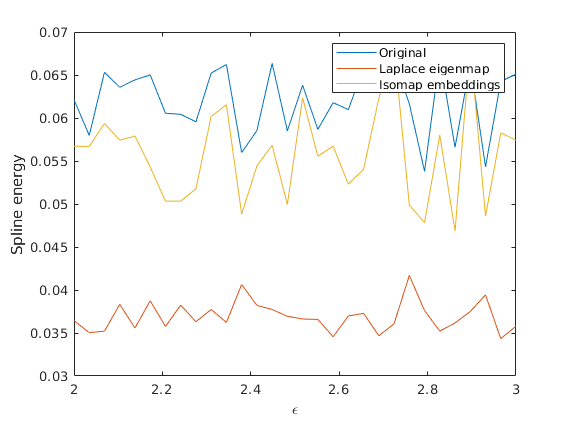
\includegraphics[scale=0.6]{figure/p3.png}
	\caption{spline energy versus $\epsilon$}
	\label{fig1}
\end{figure}

The figure shows that Laplace eigenmap results in the smoothest representation of $f$.
\end{document}
